\def\layersep{2.5cm}

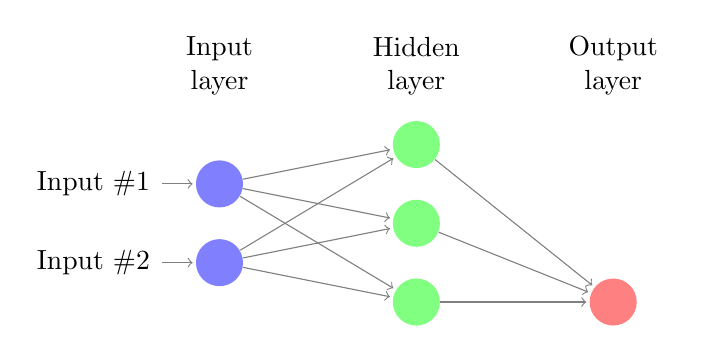
\begin{tikzpicture}[shorten >=1pt,->,draw=black!50, node distance=\layersep]
    \tikzstyle{every pin edge}=[<-,shorten <=1pt]
    \tikzstyle{neuron}=[circle,fill=black!25,minimum size=17pt,inner sep=0pt]
    \tikzstyle{input neuron}=[neuron, fill=blue!50];
    \tikzstyle{output neuron}=[neuron, fill=red!50];
    \tikzstyle{hidden neuron}=[neuron, fill=green!50];
    \tikzstyle{annot} = [text width=4em, text centered]

    % Draw the input layer nodes
    \foreach \name / \y in {1,...,2}
    % This is the same as writing \foreach \name / \y in {1/1,2/2,3/3,4/4}
        \node[input neuron, pin=left:Input \#\y] (I-\name) at (0,-\y) {};

    % Draw the hidden layer nodes
    \foreach \name / \y in {1,...,3}
        \path[yshift=0.5cm]
            node[hidden neuron] (H-\name) at (\layersep,-\y cm) {};

    % Draw the output layer node
    %\node[output neuron,pin={[pin edge={->}]right:Output}, right of=H-3] (O) {};
    \node[output neuron, right of=H-3] (O) {};

    % Connect every node in the input layer with every node in the
    % hidden layer.
    \foreach \source in {1,...,2}
        \foreach \dest in {1,...,3}
            \path (I-\source) edge (H-\dest);

    % Connect every node in the hidden layer with the output layer
    \foreach \source in {1,...,3}
        \path (H-\source) edge (O);

    % Annotate the layers
    \node[annot,above of=H-1, node distance=1cm] (hl) {Hidden layer};
    \node[annot,left of=hl] {Input layer};
    \node[annot,right of=hl] {Output layer};   

  %   \node[annot,below of=H-5, node distance=2cm] (hk) {
  %       \[%Matrix Input    
		% \begin{pmatrix}
		% h_{1, 1} \\
		% h_{1, 2} \\
		% h_{1, 3} \\
		% \vdots \\
		% h_{1, m} 
		% \end{pmatrix}\]
  %   };

  %   \node[annot,left of=hk] {
  %   	\[\begin{pmatrix}
		% 1 \\
		% x_{1} \\
		% x_{2} \\
		% \vdots \\
		% x_{m} 
		% \end{pmatrix}\]
  %   };
  %   \node[annot,right of=hk] {
  %   	\[\begin{pmatrix}
		% y_{1} \\
		% y_{2} \\
		% \vdots \\
		% y_{m} 
		% \end{pmatrix}\]
  %   };

\end{tikzpicture}
